\documentclass{article}
\usepackage{amsmath, graphicx}
\usepackage[a4paper, margin=2cm]{geometry}

\title{Euler Equations}
\begin{document}
\maketitle

The Euler equations are the fundamental model for describing the motion of an
\emph{inviscid, compressible fluid}, i.e.\ a fluid without viscosity or heat conduction.  
They are derived from the basic conservation laws applied to a fluid element:

\begin{itemize}
  \item \textbf{Mass conservation (continuity):}
  \[
  \frac{\partial \rho}{\partial t} + \nabla \cdot (\rho \mathbf{u}) = 0
  \]

  \item \textbf{Momentum conservation (Newton's second law):}
  \[
  \frac{\partial (\rho \mathbf{u})}{\partial t} 
  + \nabla \cdot \big(\rho \mathbf{u} \otimes \mathbf{u} + p I \big) = 0
  \]

  \item \textbf{Energy conservation:}
  \[
  \frac{\partial E}{\partial t} 
  + \nabla \cdot \big[(E+p)\mathbf{u}\big] = 0
  \]
\end{itemize}
Here $\rho$ is the density, $\mathbf{u}$ the velocity vector, $p$ the pressure, and $E$ the total energy density. They describe nonlinear wave phenomena such as shocks, rarefactions, and contact discontinuities. 

\section*{Euler Equations in Primitive Variables}

The Euler equations in primitive variables $q = (\rho, u, p)^T$ are:
\begin{align}
\frac{\partial \rho}{\partial t} + u \frac{\partial \rho}{\partial x} + \rho \frac{\partial u}{\partial x} &= 0 \label{eq:euler1} \\[6pt]
\frac{\partial u}{\partial t} + u \frac{\partial u}{\partial x} + \frac{1}{\rho} \frac{\partial p}{\partial x} &= 0 \label{eq:euler2} \\[6pt]
\frac{\partial p}{\partial t} + u \frac{\partial p}{\partial x} + \gamma p \frac{\partial u}{\partial x} &= 0 \label{eq:euler3}
\end{align}
This system can be written compactly as
\begin{equation}
q_t + A(q) q_x = 0, 
\qquad 
A(q) =
\begin{pmatrix}
u & \rho & 0 \\
0 & u & 1/\rho \\
0 & \gamma p & u
\end{pmatrix}.
\end{equation}

\subsection*{Eigenvalues (Wave Speeds)}
The eigenvalues of $A(q)$ are
\begin{equation}
\lambda^{(-)} = u - c, 
\qquad \lambda^{(0)} = u, 
\qquad \lambda^{(+)} = u + c,
\end{equation}
where the sound speed is
\begin{equation}
c = \sqrt{\frac{\gamma p}{\rho}}.
\end{equation}


\subsection*{Right Eigenvectors}

The corresponding right eigenvectors are
\begin{equation}
r^{(-)} =
\begin{pmatrix}
1 \\[4pt] -c/\rho \\[4pt] c^2
\end{pmatrix},
\qquad
r^{(0)} =
\begin{pmatrix}
1 \\[4pt] 0 \\[4pt] 0
\end{pmatrix},
\qquad
r^{(+)} =
\begin{pmatrix}
1 \\[4pt] c/\rho \\[4pt] c^2
\end{pmatrix}.
\end{equation}

\subsection*{Left Eigenvectors}

The left eigenvectors (the eigenvectors of $A^\mathrm{T}$), normalized such that $l_i \cdot r_j = \delta_{ij}$, are
\begin{equation}
l^{(-)} = 
\begin{pmatrix}
0 & -\tfrac{\rho}{2c} & \tfrac{1}{2c^2}
\end{pmatrix},
\qquad
l^{(0)} = 
\begin{pmatrix}
1 & 0 & -\tfrac{1}{c^2}
\end{pmatrix},
\qquad
l^{(+)} = 
\begin{pmatrix}
0 & \tfrac{\rho}{2c} & \tfrac{1}{2c^2}
\end{pmatrix}.
\end{equation}

\subsection*{Characteristic Form}

Let $R = (r^{(-)}\;|\;r^{(0)}\;|\;r^{(+)})$ be the matrix of right eigenvectors ($R$ is a square matrix whose columns are the eigenvectors), and $L = R^{-1}$ the matrix of left eigenvectors. Then
\begin{equation}
L A R = \Lambda = \mathrm{diag}(u-c, \; u, \; u+c).
\end{equation}
Defining the characteristic variables $w = L q$ (is equivalent to $\mathrm{d}w = L\mathrm{d}q$), the system diagonalizes:
\begin{align}
w^{(-)}_{t} + (u-c) w^{(-)}_{x} &= 0, \\
w^{(0)}_{t} + u w^{(0)}_{x} &= 0, \\
w^{(+)}_{t} + (u+c) w^{(+)}_{x} &= 0.
\end{align}
Each is a simple advection equation of the form
\[
\frac{\partial w}{\partial t} + \lambda \frac{\partial w}{\partial x} = 0.
\]
The characteristic curves are defined by
\[
\frac{dx}{dt} = \lambda,
\]
with $\lambda = u-c$, $u$, $u+c$.
Along these curves, the total derivative vanishes:
\[
\frac{d w}{dt} = \frac{\partial w}{\partial t} + \frac{dx}{dt}\frac{\partial w}{\partial x}
= w_t + \lambda w_x = 0.
\]{(0)}
So indeed,
\[
w = \text{constant along } \frac{dx}{dt} = \lambda.
\]


\section*{The Riemann Problem}
The \emph{Riemann problem} consists of two constant states (left and right) separated
by a discontinuity at an interface. For the Euler equations, the system is nonlinear
and has three eigenvalues:
\[
\lambda^{(-)} = u - c, \qquad
\lambda^{(0)} = u, \qquad
\lambda^{(+)} = u + c ,
\]
corresponding to three distinct waves that emerge from the interface. As time evolves, these three waves propagate outward, dividing the domain into four regions
\[
\text{Left (L)} \;\;|\;\; \text{Left-star (L$_*$)} \;\;|\;\;
\text{Right-star (R$_*$)} \;\;|\;\; \text{Right (R)}.
\]
see FIG. \ref{fig:riemann-problem}

\begin{figure}[h]
    \centering
    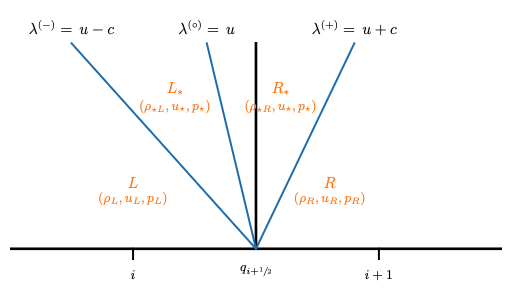
\includegraphics[width=0.7\textwidth]{figures/riemann-problem.png}
    \caption{Schematic of the Riemann problem for the Euler equations. 
    An initial discontinuity between left (L) and right (R) states evolves 
    into three waves: a left-moving acoustic wave ($u-c$), a contact 
    discontinuity ($u$), and a right-moving acoustic wave ($u+c$). 
    These divide the domain into four regions: L, L$_*$, R$_*$, and R.}
    \label{fig:riemann-problem}
\end{figure}


\paragraph{Wave types:}
\begin{itemize}
  \item The \textbf{middle wave} ($\lambda^{(0)} = u$) is a \emph{contact discontinuity}.  
        It separates two states but has constant velocity and pressure across it.  
        Only density can jump across this wave (we know this from the eigenvectors $r^{(0)}=(1,0,0)^\mathrm{T}$).
  \item The \textbf{left} ($u-c$) and \textbf{right} ($u+c$) waves can each be either
        a \emph{shock} (if the flow is compressing) or a \emph{rarefaction} (if expanding).
\end{itemize}
The solution of the Riemann problem reduces to finding the pressure and velocity
in the intermediate (star) region:
\[
(p_*, u_*),
\]
together with the corresponding left- and right-star densities $\rho_{*L}, \rho_{*R}$. Thus, the Riemann problem solution consists of:
\begin{enumerate}
  \item Determining the wave structure (shock or rarefaction) for each side.
  \item Solving for the intermediate state $(p_*, u_*)$.
  \item Constructing the full piecewise solution across the three waves.
\end{enumerate}

\subsection*{Rarefaction Waves}

Across a rarefaction, the flow is expanding rather than compressing.  To analyze this, we consider the primitive variables with entropy,
\[
q_s = (\rho, u, s)^\mathrm{T}.
\]
Here, the Euler equations in primitive variables $(\rho, u, p)$ close the system if we already assume an equation of state (EOS), e.g. ideal gas $p = (\gamma-1)\rho e$. But when we want to describe wave phenomena (shocks, rarefactions), we also need to know how entropy behaves, because across shocks entropy increases, and across rarefactions entropy remains constant. Therefore, for rarefaction, the entropy satisfies
\[
\frac{Ds}{Dt} = 0.
\]
Therefore, we have
\[
\frac{Ds}{Dt} = \frac{\partial s}{\partial t} + \frac{\mathrm{d}x}{\mathrm{d}t}\frac{\partial s}{\partial x} = \frac{\partial s}{\partial t} + u\frac{\partial s}{\partial x} = 0
\]
Using $p = p(\rho,s)$, we write
\begin{equation}
\frac{\partial p}{\partial x} =
\left.\frac{\partial p}{\partial s}\right|_{\rho}\frac{\partial s}{\partial x}
+ \left.\frac{\partial p}{\partial \rho}\right|_{s}\frac{\partial \rho}{\partial x}
= \left.\frac{\partial p}{\partial s}\right|_{\rho}\frac{\partial s}{\partial x}
+ \frac{p \Gamma_1}{\rho}\frac{\partial \rho}{\partial x},
\end{equation}
where $\Gamma_1 = \left.\frac{\partial \ln p}{\partial \ln \rho}\right|_s$ is the adiabatic index. So the system can be written as
\begin{equation}
(q_s)_t + A_s(q_s)\,(q_s)_x = 0,
\qquad
A_s(q_s) =
\begin{pmatrix}
u & \rho & 0 \\
c^2/\rho & u & 1 \\
\displaystyle \rho\,\left.\frac{\partial p}{\partial s}\right|_{\rho} & 0 & u
\end{pmatrix},
\label{eq:entropy-form}
\end{equation}
The eigenvalues of $A_s(q_s)$ are still
\[
\lambda_{-} = u - c,\qquad \lambda_{0} = u,\qquad \lambda_{+} = u + c .
\]
These coincide with the primitive $(\rho,u,p)$ form because the physics is the same. A convenient choice of right eigenvectors is
\begin{equation}
r^{(-)}_s =
\begin{pmatrix}
1 \\[2pt] -\,c/\rho \\[2pt] 0
\end{pmatrix},
\qquad
r^{(0)}_s =
\begin{pmatrix}
1 \\[2pt] 0 \\[2pt] -\,c^2/p_s
\end{pmatrix},
\qquad
r^{(+)}_s =
\begin{pmatrix}
1 \\[2pt] c/\rho \\[2pt] 0
\end{pmatrix}.
\label{eq:right-eig-entropy}
\end{equation}
In this basis, entropy does not change across the acoustic waves ($r^{(\pm)}_s$ have zero $s$‑component), while the middle wave is the entropy/contact mode. 

\subsection*{Characteristic Conditions Across a Rarefaction}
Consider the $(-)$ wave, which moves at a speed $\lambda^{(-)}=u-c$. Across this wave, the characteristic variable $w^{(-)}$ will jump, but $w^{(0)}$ and $w^{(+)}$ will not. So we can use this constancy to tell us how the evolution behaves across that wave $w^{(-)}$. The constancy of the middle and right characteristic variables across the left wave gives us the conditions:
\[
l^{(+)}.\mathrm{d}q=0, \quad l^{(0)}.\mathrm{d}q=0
\]
gives
\begin{align}
du + \frac{1}{\rho c}\, dp &= 0, \label{eq:left-rare-u} \\
d\rho - \frac{1}{c^2}\, dp &= 0. \label{eq:left-rare-rho}
\end{align}
Similar arguments would give the condition across the right wave as:
\begin{align}
du - \frac{1}{\rho c}\, dp &= 0, \\
d\rho - \frac{1}{c^2}\, dp &= 0.
\end{align}

\paragraph{Lagrangian form.}
Defining specific volume $\tau = 1/\rho$ and Lagrangian sound speed $C=\rho c$,
these become
\[
du = \pm \frac{dp}{C}, 
\qquad d\tau = -\frac{dp}{C^2},
\]
with the upper sign for the left wave and the lower sign for the right wave.

\paragraph{$\gamma$-law gas.}
For a $\gamma$-law gas, $p=K\rho^\gamma$, where $K$ is a constant that depends on the entropy, and we can integrate explicitly to obtain the \emph{Riemann invariants}:
\[
u \mp \frac{2c}{\gamma-1} = \text{constant along } \frac{dx}{dt} = u \pm c.
\]

\medskip
\noindent
Hence, across a rarefaction:
\begin{itemize}
  \item entropy remains constant,
  \item pressure, density, and velocity vary smoothly according to the 
        characteristic relations,
  \item the solution forms a continuous ``fan'' bounded by $u \pm c$.
\end{itemize}
Applying this between the left state $(\rho_L,u_L,p_L)$ and the star region $(\rho_\star,u_\star,p_\star)$ yields
\begin{equation}
u_L + \frac{2c_L}{\gamma-1} \;=\; u_\star + \frac{2c_\star}{\gamma-1}.
\label{eq:left-rarefaction-invariant}
\end{equation}
Together with the constant-entropy EOS
\begin{equation}
\frac{p_L}{\rho_L^\gamma} = \frac{p_\star}{\rho_\star^\gamma},
\end{equation}
this leads to an explicit relation
\begin{equation}
u_{\star,L} = u_L + \frac{2c_L}{\gamma-1}
\left[ 1 - \left(\frac{p_\star}{p_L}\right)^{\frac{\gamma-1}{2\gamma}} \right].
\label{eq:u-star-L}
\end{equation}
A similar construction across the right state gives
\begin{equation}
u_{\star,R} = u_R - \frac{2c_R}{\gamma-1}
\left[ 1 - \left(\frac{p_\star}{p_R}\right)^{\frac{\gamma-1}{2\gamma}} \right].
\label{eq:u-star-R}
\end{equation}
Here $u_{\star,L}$ and $u_{\star,R}$ represent the star-region velocity
as predicted from the left and right states, respectively.
Physically, the star region has a single velocity $u_\star$, so we require
\begin{equation}
u_{\star,L} \;=\; u_{\star,R} \;\equiv\; u_\star,
\end{equation}
which provides the condition to solve for the unknown pressure $p_\star$ and velocity $u_\star$ in the Riemann problem.




\end{document}